\documentclass[./thesis.tex]{subfiles}

\newcommand{\Gpqrs}{\ket{G^{rs}_{pq}}}
\begin{document}
\label{chap:CIPSI}


\begin{algorithm}
	\label{alg:cipsi_manu}
	\caption{Simple CIPSI}
		\KwData{ $\ket \Psi$ }
		\KwResult{ Guarantees all $\epsilon(\alpha)$ are computed a single time. }
		sort $\ket {D_i}$ by decreasing ${c_i}^2$ \;
		\For {$g \gets 1, N_{gen}$}{
		\tcc{apply all double excitations on $|D_g \rangle$}
		\ForAll {$\ket \alpha$ ; $\langle D_g | H | \alpha \rangle \neq 0$}{
		\For{$p \gets 1, g-1$}{
			\If{$\ket \alpha$ connected to $\ket {D_p}$}{
				\tcc{$\ket \alpha$ has already been generated by $\ket {D_p}$}
				discard this $\ket \alpha$ \;
			}
		}
		search $\kalpha$ in $D_{N_{sel}+1},\ldots,D_{\Ndet}$ \;
		\If{$\kalpha$ was found}{
			discard this $\kalpha$
		}
		 $R \gets 0$ \;
		\For{$s \gets g, N_{sel}$}{
			$R \gets R + \Hij{D_s}{\alpha}$ \;	
			\tcc{$\ket {D_s}==\kalpha$ is noticed when computing $\Hij{D_s}{\alpha}$}	
			\If{$\ket {D_s}==\kalpha$}{
				\tcc{$\kalpha \in \Psi$}
				discard this $\ket \alpha$
			}
		}
		 assert $R == \Hij{\Psi}{\alpha}$  \;
		 $\epsilon(\alpha) = \frac{R^2}{\Delta E_\alpha}$
		}
		}
\end{algorithm}




\section{def}

My initial and most important work has been the improvement of the CIPSI algorithm present in the Quantum Package, that had been implemented by my predecessor\cite{giner:tel-01077016}. As was briefely described in the previous chapter, it is an \emph{on the fly} iterative selection algorithm, where determinants are added to the variational wavefunction according to a perturbative criterion. Because it gathers a large amount of information, this CIPSI algorithm has been the basis for other subsequent works presented in the next chapters.

Iteration $n$ of CIPSI can be described like so:

\begin{enumerate}
\item

The variational function $\ket {\Psi^{(n)}}$ is defined over a set of determinants $  \mathcal{D}^{(n)}$ in which we diagonalize $\widehat{H}$
\begin{equation}
\ket{\Psi^{(n)}} = \sum_{S \in \mathcal{D}^{(n)}} c_S^{(n)} \ket{S}
\end{equation}

\item
For all $\kalpha \notin \mathcal{D}^{(n)}$, we compute a perturbative contribution
\begin{equation}
e_\alpha = \frac{\Hij{\Psi^{(n)}}{\alpha}^2}{E^{(n)} - H_{\alpha \alpha}}
\end{equation}
$E^{(n)}$ is an energy that depends on the pertubation theory being used. In our case, the Epstein-Nesbet energy is used.

\item
From $\{ \alpha \}^{(n)}$ the set of all $\kalpha$ considered at current iteration, we extract $\{ \alpha^\star \}^{(n)}$ the set of $\kalpha$ of highest contributions $e_\alpha$, and add them to the wavefunction
\begin{equation}
\mathcal{D}^{(n+1)} = \mathcal{D}^{(n)} \cup \{ \alpha^\star \}
\end{equation}

\item
$\EFCI$ energy can be estimated
\begin{equation}
\EFCI \approx E^{(n)}_0 + E_{PT2}^{(n)}
\end{equation}


with $E^{(n)}_0$ the variational energy of $\ket {\Psi^{(n)}}$ and
\begin{equation}
E_{PT2}^{(n)} = \sum_{\alpha \in \{\alpha \}^{(n)}} e_\alpha
\end{equation}
\item
Exit on some criterion (number of determinants in the wavefunction, low $\EPT^{(n)}$...).

\end{enumerate}



As can be seen, CIPSI involves creation of an external space and precise knowledge of how it interacts with the internal space. Algorithmically speaking, we will need to enumerate all connections between all internal and all external determinants.
There are, perhaps schematically, two ways to do this :

\begin{itemize}
\item
``external to internal'', looping over all possible $\kalpha$ and computing $e_\alpha$.
\item
``internal to external'', looping over all internal determiants $\ket G$ and all double excitations $\hat T$, creating $\kalpha = \hat T \ket G$, then incrementing $\tilde e_{\alpha \notin \Psi}$ by $\Hij{G}{\alpha}$. Finally get $e_{\alpha \notin \Psi} = \frac{\tilde e_\alpha}{E^{(n)} - H_{\alpha \alpha}}$
\end{itemize}

While the later approach sounds more efficient, it has the obvious issue of requiring all $e_\alpha$ to be stored in memory simultaneously. Unfortunately this is usually not feasible, since their numbers scales as $\Ndet \times \mathcal{O}_{virt}^2 \times \mathcal{O}_{occ}^2$.
While the later approach is simpler, it begs the question of how to generate all possible $\kalpha$ not simultaneously and with no duplicates. 


\section{Approximation}

Given the qualitative nature of this procedure - each $\kalpha$ is either selected or not - it is possible to save a vast amount of computation with minimal approximations. These were present in the original version and retained in the new one.

Both the former and newer version of CIPSI generates the external space in a ``internal to external'' way, that is, by applying double excitations to determinants of $\Psi$ ; a determinant used for creation of $\kalpha$ is refered to as a \emph{generator}.

Ensuring each $\epsilon(\alpha)$ is considered only once, is done by checking all newly generated $\kalpha$ for connection (at most double excitation) to a determinant $\ket {D_i}$ previously used as a generator ; if a connection $\hat T$ is found, it means $\kalpha$ was already generated from $\ket {D_i}$ as $\hat T \ket {D_i}$.

Determinants $D_I \in \Psi$ are sorted by decreasing absolute values of $c_I$. Two approximations are made :

\begin{itemize}
\item
It is very unlikely $\ket \alpha$ will be selected if it's not connected to any $\ket D$ with a large coefficient. Therefore, it is possible to only consider the determinants of larger coefficent as generators. We choose a number of generators $N_{gen}$ and only consider $D_{I \leq N_{gen}}$ as generators. In practice we set $N_{gen}$ according to a norm threshold $n_g$, picking $N_{gen}$ as the highest value fullfilling
\begin{equation}
\sum_{I \leq N_{gen}} c_I^2 \leq n_g
\end{equation}
\item
Connections to $\ket {D_i}$ of small coefficient can be neglected. We do not need accurate values for $\epsilon(\alpha)$, small differences are unlikely to substantially change the subset of the largest ones. This approximation is achieved in a similar way by defining $N_{sel} \leq \Ngen$ a number of so-called \emph{selectors}, and approximating
\begin{equation}
  \Hij{\Psi}{\alpha} \approx \sum_{i \leq N_{sel}} c_i \Hij{D_i}{\alpha}
\end{equation}

\end{itemize}

Note that generator determinants are a subset of selector determinants. See figure \ref{fig:generators_selectors}.


\begin{figure}[h!]
	
	\begin{center}
		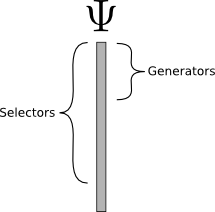
\includegraphics[width=0.4\columnwidth]{figures/cipsi/selexemple2}
		\caption{$\ket \Psi$ is sorted by decreasing ${c_I}^2$; generator and selector subsets are defined.}
		\label{fig:generators_selectors}
	\end{center}
\end{figure}



\section{Original version}

Originally, the Quantum Package generated the external space in a ``internal to external'' way, by applying all excitations on all determinants ; but the computation of $e_\alpha$ itself was a straighforward ``external to internal'', computing a single $e_\alpha$ at a time, avoiding the problem of keeping track of all $\epsilon(\alpha)$ simultaneously.

While this version is obsolete, since it is relatively simple, it is briefly presented for pedagogic reasons. A slightly more detailed algorithmic version is shown as algorithm \ref{alg:cipsi_manu}.

\begin{enumerate}
\item
$\ket {D_i}$ are sorted with decreasing ${c_I}^2$.
\item
loop over generators $\ket G$
\item
generate all determinants connected to $G$
\item
from this set, discard those that appear in $\Psi$. This is now a set of $\ket \alpha$
\item
from this set, discard those that have already been generated before, i.e. those connected to $D_K$ with $K<I$. This is now a set of unique $\ket \alpha$.
\item
compute $\epsilon(\alpha) = \frac{\langle \alpha|H|\Psi\rangle^2}{\Delta E_\alpha}$ for those new $\ket \alpha$
\end{enumerate}


\section{Current version base idea}

The current approach is intermediate between computing $\epsilon(\alpha)$ one by one, and keeping track of all of them at the same time.
It creates a subset, or ``batch'' of determinants small enough to fit into memory, and importantly, that isn't arbitrary.
A batch is defined by a doubly ionized generator


\begin{equation}
\ket {G_{pq}} = a_p a_q \ket G
\end{equation}



Determinants contained in the $\ket {G_{pq}}$ batch , some of which may be unique $\kalpha$, can be systematically defined by two indexes $r$ and $s$ with

\begin{equation}
a^\dagger_r a^\dagger_s a_p a_q  \ket G = \Gpqrs
\end{equation}

Essentially, determinants in a batch are defined by their difference to $G_{pq}$. Therefore, comparing $G_{pq}$ to a selector determinant, allows to systematically determine which $\kalpha$ of the batch it will connect to, and by what excitation. Additional filtering mechanisms are set up to avoid considering selectors that do not interact with the current batch. Those will be explicited later on. Comparing figures \ref{fig:old_cipsi} and \ref{fig:new_cipsi} hints the differences between the former an newer algorithm. Note that because generators are a subset of selectors, a particular $\kalpha$ generated from $\ket {D_g}$ must be checked for connection to all selectors either as generators or as selectors.

\begin{itemize}
\item
$\ket {D_{I \in [1,g-1]}}$ as generators to check if $\kalpha$ has been previously generated
\item
$\ket {D_{I \in [g,N_{sel}]}}$ as selectors to compute $\Hij{\Psi}{\alpha}$
\end{itemize}


\begin{figure}[h!]
	\begin{center}
		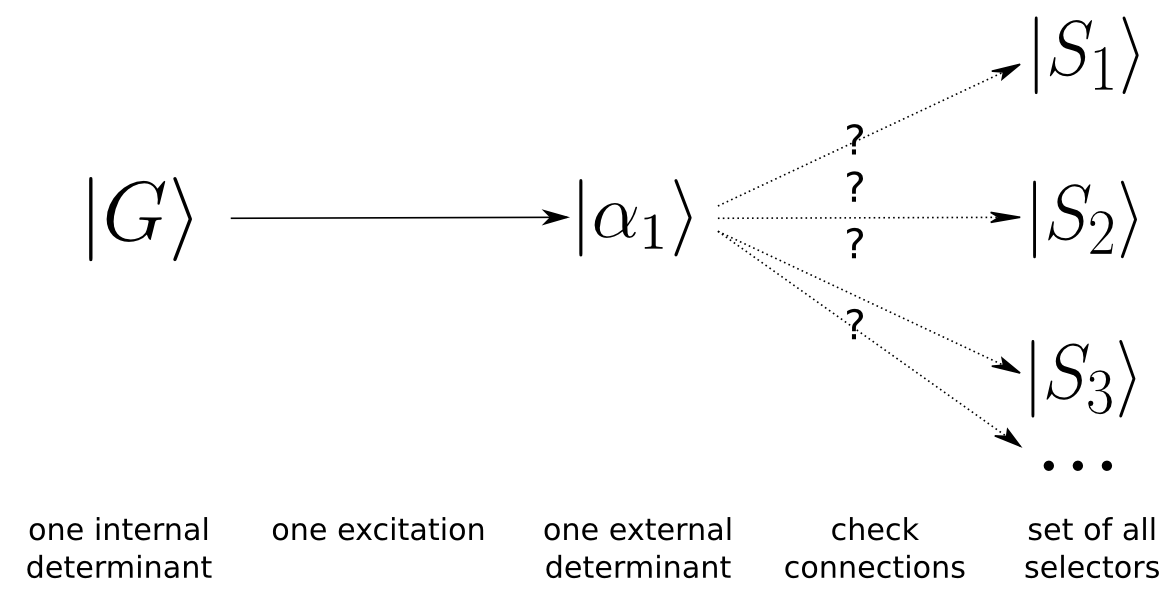
\includegraphics[width=0.7\columnwidth]{figures/cipsi/old_cipsi}
		\caption{Original CIPSI schematic representation, some details omitted}
		\label{fig:old_cipsi}
	\end{center}
\end{figure}


\begin{figure}[h!]
	\begin{center}
		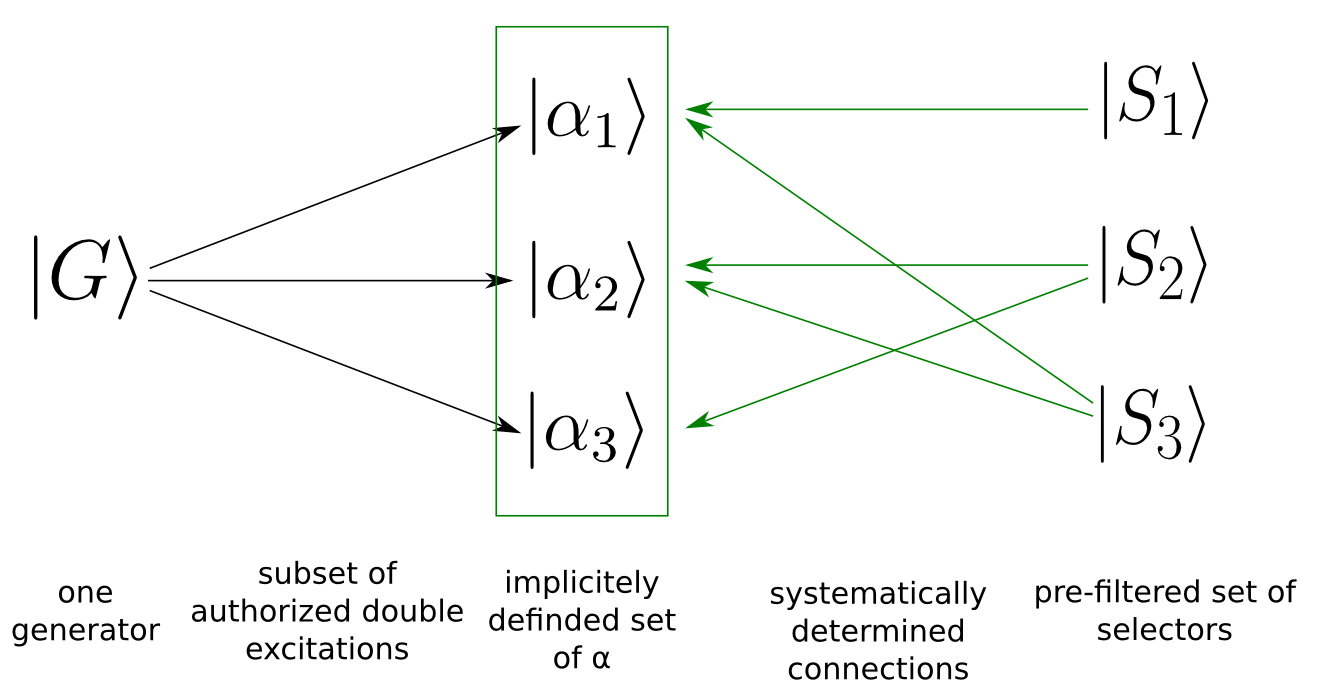
\includegraphics[width=0.7\columnwidth]{figures/cipsi/new_cipsi}
		\caption{New CIPSI schematic representation, some details omitted}
		\label{fig:new_cipsi}
	\end{center}
\end{figure}

\subsection{Unfiltered algorithm}

Filtering of selectors is a somewhat natural idea that was actually implemented before the batch approach. It however can easily be understood as something added ``on top'' of it, so it will be detailed in the next section and ignored in this one.



\begin{enumerate}
%\setlength{\itemindent}{2em}
\item
Iterate over $\ket {D_{I \leq \Ngen}} = \ket G$
\item
Iterate over all possible $a_p a_q \ket G = \ket {G_{pq}}$
\item
allocate a null matrix $P(G_{pq})$ indexed by $r$ and $s$. Each cell is associated with $a^\dagger_r a^\dagger_s a_p a_q  \ket G = \Gpqrs$. Some cells will be tagged as not being associated with a unique $\ket \alpha$, but either one of :
\begin{itemize}
\item
a determinant already present in the wavefunction
\item
a non-existing determinant, i.e. $\Gpqrs = 0$
\item
a non-unique $\ket \alpha$ (either a bi-excitation of a previous generator, or a single excitation of the current one)
\end{itemize}

\item
Since two electrons cannot occupy the same spinorbital, tag cells where $r$ or $s$ is occupied in $\ket {G_{pq}}$.
\item
Apply single excitation tagging. This ensures single excitations of $\ket G$ are generated exactly once. It is described in section \ref{single_tagging}.
\item
\textbf{selector loop}: Iterate over $\ket {D_J} = \ket S$ 
\item
Determine whether there is an $r,s$ pair so that $\ket S = \ket {G_{pq}^{rs}}$. In other words, look for $\ket S$ in the current batch. If there is, tag the corresponding cell.
\item
Determine $r,s$ pairs so that $\ket {G_{pq}^{rs}}$ is connected to $\ket S$
\item
If $J<I$, tag the corresponding cells ; $\ket {G_{pq}^{rs}}$ has already been generated by $\ket {D_J}$.
\item
If $J \geq I$, increment all untagged $P_{r,s}(G_{pq})$ matrix element by $\Delta P_{r,s}(G_{pq}) = c_J \Hij{S}{G^{rs}_{pq}}$. Note that $\overrightarrow{T}$ so that $\ket S=\overrightarrow{T} \Gpqrs$ can be determined at the same time as the $r,s$ pair.
\item
End \textbf{selector loop}. All untagged cells are guaranteed to be associated with a unique $\ket \alpha$ and $P_{r,s}(G_{pq}) = \langle \Psi |H|G^{rs}_{pq} \rangle$. $\epsilon(\alpha)$'s for the current batch can be computed  \\

\begin{equation}
\epsilon(\ket {G_{pq}^{rs}}) = \frac{P_{r,s}(G_{pq})^2}{\Delta E_{\Gpqrs}}
\end{equation}
\item
End of other loops. All $\epsilon(\alpha)$ have been computed a single time.

\end{enumerate}


\subsection{Tagging}

Tagged cells are simply tracked using a logical matrix $B(G_{pq})$ with $B_{r,s}(G_{pq})$ keeping the tag status of $\Gpqrs$, defaulting to $\text{FALSE}$. 
In some cases, full columns/rows are to be tagged. Keeping track of fully tagged rows or column is useful for performance purpose, as it allows to shortcut some loops. A simple way to do it, is to add an extra column and an extra row of index $0$ to $B$ ; $B_{0,s}(G_{pq}) = \text{TRUE}$ means the whole $s$ column is tagged, $B_{r,0}(G_{pq}) = \text{TRUE}$ means the whole $s$ line is tagged. The actual tag status of $\Gpqrs$ becomes
\begin{equation}
B_{r,0}(G_{pq}) \vee B_{0,s}(G_{pq}) \vee B_{r,s}(G_{pq})
\end{equation}
While significant, this optimization is fairly simple to set up and use, so for simplification purpose, it will be ignored.


\subsection{Single excitation tagging}
\label{single_tagging}
The algorithm is designed to generate all $\ket {G_{pq}^{rs}}$, which are doubly excited from $\ket G$. The singly excited determinants are not explicitly generated, but are formally present as $\ket{G_{pq}^{ps}}$.
The issue is that $\ket{G_{pq}^{ps}}$ refers to the same determinant $a^\dagger_s a_q \ket{G}$ regardless of $p$, and the base algorithm only tags a $\kalpha$ as duplicate if it has a previous generator $\ket K$, i.e. if

\begin{equation}
\ket {G_{pq}^{rs}} = \ket {K_{p'q'}^{r's'}} ; K = D_{I'<I}
\end{equation}

As can be seen this doesn't cover the case where $G_{pq}^{ps} = G_{p'q}^{p's}$.

To solve this issue, we default to tag $G_{pq}^{ps}$, which prevents generating single excitations, and selectively untag in certain cases:


\begin{itemize}
\item
\textbf{Untagging all $\alpha$ single excitations of $\ket G$ exactly once}:

Pick $P$ any ``non-frozen'' $\beta$ spinorbital occupied in $\ket G$. We arbitrarily choose the lowest one. Untag $\ket {G_{Pq}^{Ps}}$ whenever $q,s$ are of spin $\alpha$. Any $\alpha$ single excitation $q \rightarrow  s$ is untagged a single time.

$P$ cannot be chosen of spin $\alpha$, because single excitations $P \rightarrow  s$ and $q \rightarrow  P$ would be formally present as $G_{PP}^{Ps}$ and $G_{Pq}^{PP}$, which aren't ever generated, since for obvious reasons the base algorithm never considers $G_{qq}$ or $G_{pq}^{rr}$.
\item
\textbf{Untagging all $\beta$ single excitations of $\ket G$ exactly once}:

Pick $Q$ any $\alpha$ spinorbital occupied in $\ket G$ - again we arbitrarily choose the lowest one. If $p,q$ are of spin $\beta$, untag $G_{pQ}^{rQ}$. Any $\beta$ single excitation $p \rightarrow  r$ is untagged a single time.
\end{itemize}


\section{Systematic determination}

The systematic determination of connections between $\ket S$ and determinants from the $\ket {G_{pq}}$ batch is done by comparing $\ket S$ to the double ionized determinant $\ket {G_{pq}}$. This yields a set of spinorbitals whose occupation status differs. Remembering $\ket S$ has two extra electrons compared to $\ket {G_{pq}}$, there are 4 cases of interest:
\begin{itemize}

\item
$i$,$j$ are occupied in $\ket S$ but not in $\ket {G_{pq}}$
\item
$i$,$j$,$k$ are occupied in $\ket S$ but not in $\ket {G_{pq}}$ ; $a$ is occupied in $\ket {G_{pq}}$, but not in $\ket S$
\item
$i$,$j$,$k$,$l$ are occupied in $\ket S$ but not in $\ket {G_{pq}}$ ; $a$,$b$ are occupied in $\ket {G_{pq}}$, but not in $\ket S$
\item
More differences : $\ket S$ isn't connected to any $\ket {G_{pq}^{rs}}$ and can be ignored. 

\end{itemize}

Based on these indices, it's possible to immediately deduce any $r,s$ pair so that $\ket {G_{pq}^{rs}}$ is at most a double excitation of $\ket S$, as well as the excitation operator $\overrightarrow{T}$ so that $\ket {G_{pq}^{rs}}=\overrightarrow{T} \ket S$. Figures \ref{fig:systematic_determination} and \ref{fig:systematic_determination2} show two possible cases as example.

While this could be done in a more compact way, we took a more case by case approach, allowing more specialized code for each situation. Taking spin into account, the different cases are listed in table \ref{tab:systematic_determination}.


It's noticeable that, because of the "wildcard" indices $X$ and $Y$ :
\begin{itemize}

\item
Cases of the form $a,ijk$ cause full rows/columns of $P(G_{pq})$ to be tagged or incremented.
\item
Cases of the form $ij$ cause the whole $P(G_{pq})$ matrix to be tagged or incremented. Obviously, tagging the whole matrix means stopping the computation for $\ket {G_{pq}}$.
\end{itemize}

\begin{figure}[h!]
	\begin{center}
		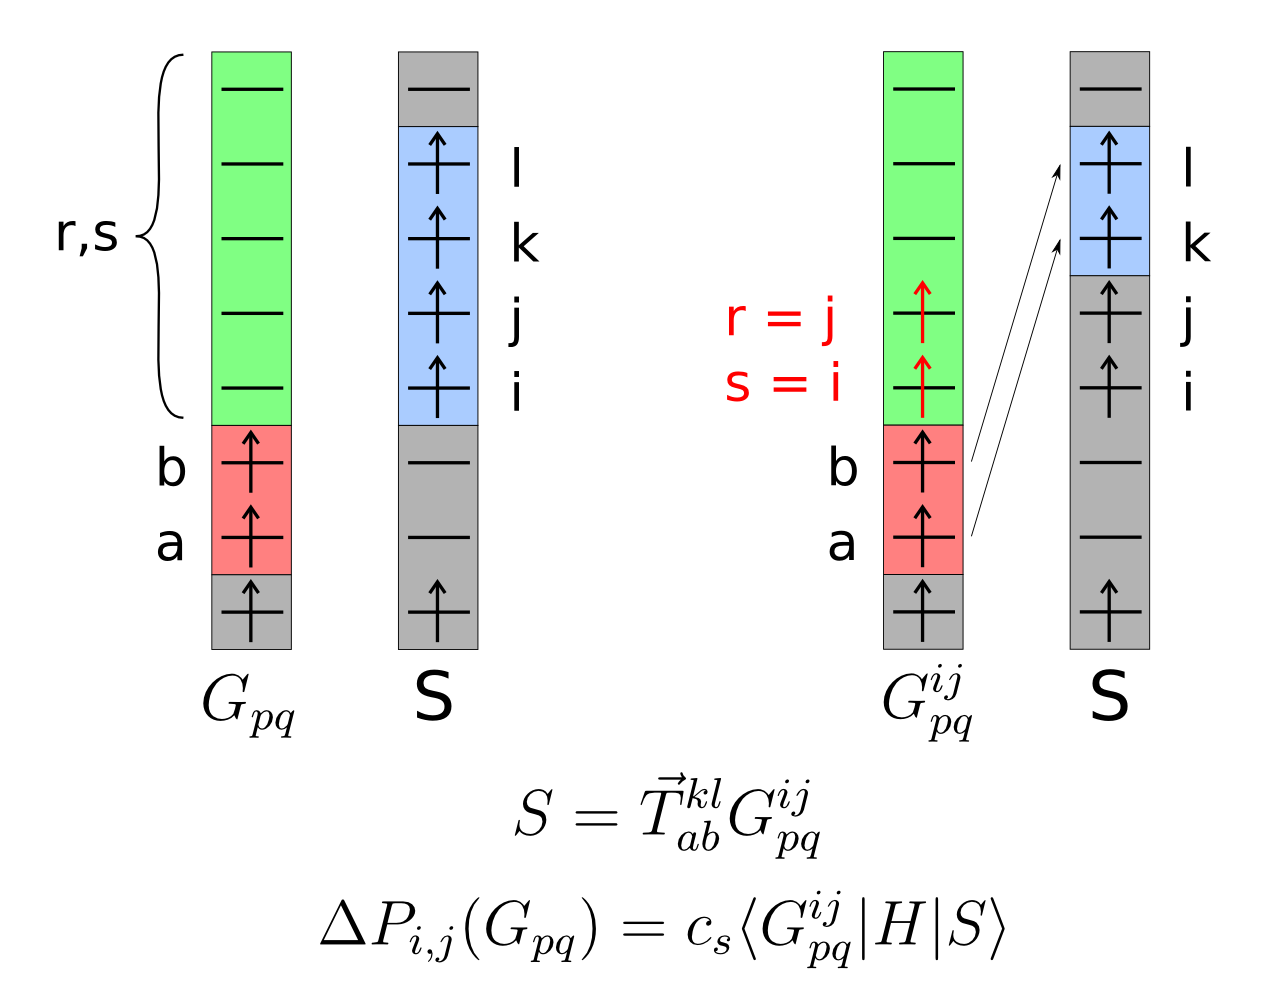
\includegraphics[width=0.70\columnwidth]{figures/cipsi/systematic_determination}
		\caption{Illustrative exemple of systematic determination of connection between a selector $\ket S$ and determinants of the $\ket {G_{pq}}$ batch when $p$ and $q$ are of same spin}
		\label{fig:systematic_determination}
	\end{center}
	
\end{figure}


\begin{figure}[h!]
	\begin{center}
		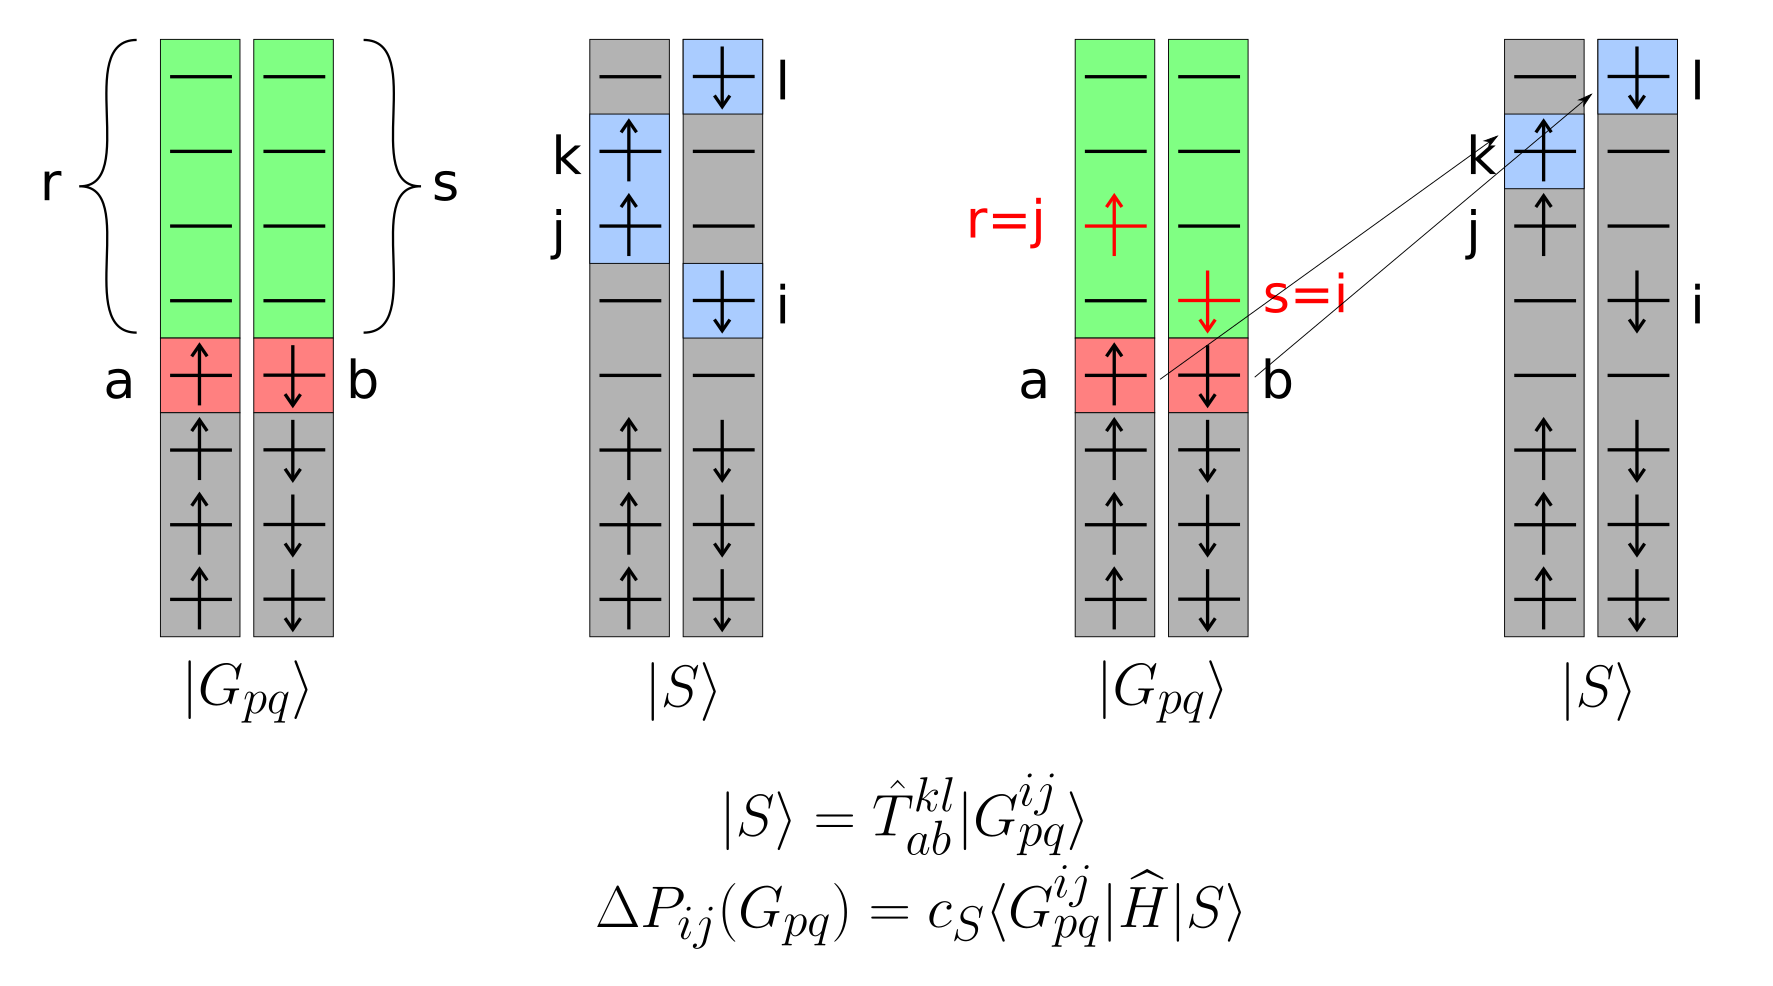
\includegraphics[width=0.70\columnwidth]{figures/cipsi/systematic_determination2}	
		\caption{Illustrative exemple of systematic determination of connection between a selector $\ket S$ and determinants of the $\ket {G_{pq}}$ batch when $p$ and $q$ are of different spin}
		\label{fig:systematic_determination2}
	\end{center}
\end{figure}



\begin{algorithm}
	\caption{simplified CIPSI}
	\label{alg:selection}
	\KwData{ $\Psi$}
	\KwResult{ $\Hij{\alpha}{\Psi} \neq 0$ has been computed exactly once for any $\alpha \notin \Psi$ }
		
	\For{$g \gets 1, t_g$}{
	$M_\alpha \gets$ any $\alpha$ spinorbital occupied in $D_g$ \;
	$M_\beta \gets$ any $\beta$ spinorbital occupied in $D_g$ \;
	\ForAll{$(p,q) ; a_p a_q D_g \neq 0$}{
		$G_{pq} \gets a_p a_q D_g$\;
		$B$ a logical matrix size $N_{sorb} \times N_{sorb}$ \;
		$P$ a real matrix size $N_{sorb} \times N_{sorb}$ \;
		\tcc{$B$ and $P$ are indexed by spinrobitals}
		$B_{*,*} \gets TRUE$ \;
		$P_{*,*} \gets 0$ \;
		\ForAll{$r ; (a_r G_{pq} = 0)$ or $(r=p)$ or $(r=q)$}{
          		$B_{*r} \gets FALSE$ \;
          		$B_{r*} \gets FALSE$ \;
		}
		
		\tcc{unblocks some elements of $B$ so that single excitations are properly generated}
		Unblock\_single($B$, p, $q$, $M_\alpha, M_\beta$)
			
				
			
		\For{$p \gets 1,N_{det}$}{
			$S \gets D_p$ \; 
			$c \gets iand(S, not(G_{pq}))$ \; 
			\If{$popcnt(c) = 2$}{
				$e \gets LIST\_FROM\_BITSTRING(c)$\; 
				$B_{e_1, e_2} \gets FALSE$\; 			  
			}			
			\tcc{see table XXX for the loops}
			\uIf{$p < g$}{
				    
				\ForAll{$(\tilde r, \tilde s) ; \Hij{S}{G_{pq}^{\tilde r \tilde s} \neq 0}$}{
				  $B_{rs} \gets FALSE$ \;
				} 
			}
			\uElseIf{$p \leq t_s$}{
				\ForAll{$(\tilde r, \tilde s) ; \Hij{S}{G_{pq}^{\tilde r \tilde s} \neq 0} ; B_{rs}$ }{
				  $P_{rs} \gets P_{rs} + \Hij{a^\dagger_r a^\dagger_s G_{pq}}{S}$ \;
				}
			}
		}
		\ForAll{$(r,s);B_{rs}$}{
		  assert $P_{rs} = \Hij{a_r^\dagger a_s^\dagger G_{pq}}{\Psi}$ \;
		}
	}
	} 
\end{algorithm}


\begin{algorithm}
	\caption{UNBLOCK\_SINGLE}
	\label{alg:unblock_single}
		\KwData{ -------}
		\KwResult{ -------------}
		

		\If{($q$ is of spin $\alpha$) and ($p=M_\beta$)}{
				$B_{*,M_\beta} \gets TRUE$ \;	
				$B_{M_\beta,*} \gets TRUE$ \;		
			}
			
			\If{($p$ is of spin $\beta$) and ($q=M_\alpha$)}{
				$B_{*,M_\alpha} \gets TRUE$ \;	
				$B_{M_\alpha,*} \gets TRUE$ \;		
			}
\end{algorithm}



\section{Filtering and loop breaking}
A great deal of processing power is lost, because every doubly ionized generator $\ket {G_{pq}}$ is compared to all selector determinants. In the vast majority of cases, it will show no connection can be made and the selector will be ignored. Thus, it's interesting to filter selector determinants in more outer loops ( generator loop, and loop over first ionization ).

This can be done using the distance $f_A^B = f_B^A$, defined as the minimal number of operations - moving, annihilating or creating an electron - that must be done to go from a determinant $\ket A$ to a determinant $\ket B$ with respectively $n_a$ and $n_b$ electrons.
Alternatively, it can be defined as the maximum between the number of anihilations and the number of creations required to go from $\ket A$ to $\ket B$.



\begin{equation}
f_A^B = \frac{||A_\alpha \oplus B_\alpha|| + ||A_\beta \oplus B_\beta|| + |n_a-n_b|}{2}
\end{equation}


Considering $\ket S$ a selector determinant and $\ket X$ a generator determinant in a state of ionization from 0 to 2 (it essentially is a wildcard for $\ket G$, $\an p \ket G$ or $\an p \an q \ket G = \ket {G_{pq}}$).

\begin{itemize}
\item
$f_X^\alpha + f_\alpha^S \geq f_X^S$
\item
$\ket \alpha$ can be generated from $\ket X$ iff $f_X^\alpha \leq 2$
\item
$\ket \alpha$ is connected to $\ket S$ iff $f_\alpha^S \leq 2$
\item
$0 \leq (f_Y^S - f_X^S) \leq 1$ with $\ket Y = a_p \ket X$
\end{itemize}

\alert{à detailler?}

From the rules above, we can deduce that given any $\ket X$ and $\ket S$, there exists a $\kalpha$ generated from $\ket X$ so that $\Hij{\alpha}{S} \neq 0$ only if $f_X^S \leq 4$.

Based on this, a filtering system can be set up, as shown on figure \ref{fig:selection}. The diagram somewhat convoluted and deserves comments.

\paragraph{Internal determinants' path}
 
A triple loop is shown

\begin{enumerate}
\item
over generators ($G$)
\item
over $p$ a first ionization ($G_p$)
\item
over $q$ a second ionization ($G_{pq}$), i.e. over batches.
\end{enumerate}

The determinants of the internal space ``flow'' from the top $\Psi$ into intermediate lists, that are fully constructed before proceeding to the inner loop, as they will be the sources of determinants for that inner loop.
A selector can only be duplicated at the node denoted by a black circle. Otherwise, it follows a single path, always going for the horizontal path if it satisfies the associated condition.
If it doesn't satisfy the condition of an horizontal path, and there is no further vertical path, it is discarded.

\paragraph{DROP instructions}
$DROP$ instructions are reached when, predictably, the current loop iteration will not yield any unique $\kalpha$. If a determinant reaches a $\text{DROP}$, the current loop iteration ends immediately.

\begin{itemize}
\item
$\text{DROP } G_{pq}$ is reached in the case where the whole $P(G_{pq})$ matrix is to be tagged, i.e. the possible values for $(r,s)$ given by table \ref{tab:systematic_determination} are two wildcards ($X,Y$ and $X,\bar Y$)

This corresponds to the case where $\ket {G_{pq}}$ has already been created from a previous generator $\ket K$, i.e. $\ket {G_{pq}} = \ket {K_{p'q'}}$, therefore for any $r,s$ we have $\ket {K_{p'q'}^{rs}} = \ket {G_{pq}^{rs}}$.\\
\item
$\text{DROP } G_{p}$, in the same fashion, is reached when $\ket {G_{p}}$ has already been created from a previous generator $\ket K$, i.e. $\ket {G_{p}} = \ket{K_{p'}}$. For any $q,r,s$ there will be $\ket {K_{p'q}^{rs}} = \ket {G_{pq}^{rs}}$, so no new $\kalpha$ will be created.
\end{itemize}


\paragraph{Left and right paths}
There is, grosso merdo, a left and a right path. The reason for this, is that we want to reach $\text{DROP}$ instructions as fast as possible. Incidently, in each loop, the implementation should prioritize operations that may cause a reach to $\text{DROP}$.

%Not trying to reach $DROP\ G_{PQ}$ means we might completely compute the $P$ matrix, only to find that the last selector determinant tags it entierly, for the reson mentioned above.
%Not trying to reach $\text{DROP } G_{P}$ means we might iterate over batches $\Gpqrs$ that are all to be "tagged out" by a single particular selector.

The first loop separates internal determinants in two disjoint categories.


\begin{itemize}
\item
Right branch : determinants that may contribute to some $P(G_{pq})$ matrix or tag previously generated $\ket \alpha$. In other words, selectors that may connect to some $\ket {G_{pq}^{rs}}$. 

\item
Left branch : Determinants that aren't selectors, but are equal to some $\ket {G_{pq}^{rs}}$. Being non-selectors, those will not be checked for connection to any $\ket {G_{pq}^{rs}}$, but they still must be checked for equality in order to ensure $\ket {G_{pq}^{rs}} \notin \Psi$
\end{itemize}
This step sets the algorithm's complexity with respect to $\Ndet$. Naively, $f_G^S$ must be computed for all pairs of internal determinants, setting the complexity to $\mathcal{O}(\Ndet^2)$. Our current implementation fastly discards $f_G^S > 4$ by using the same method as in the Davidson diagonalization, adapted to seek excitation degrees $\leq 4$ rather than $\leq 2$. The complexity is thus reduced to $\mathcal{O}(\Ndet)$.

Note that the only point of separating those two categories rather than merging them in the same list, is to avoid additional $past$ and $selector$ tests in the second loop.
%If both those lists were merged, a $selector$ condition would need to be added for reaching the right list of the second loop, and $past$ tests would be performed pointlessly on those determinants that would have gone in the left list of the first loop.
This most likely is of little interest, depending on the implementation.
%$past$ and $selector$ should at worst mean fetching an index in an array of indices, and compare it to $I$ or $N_{sel}$ respectively.
But because it's the actual implementation and because it reduces the number of operations, it is still shown.




The second loop separates again in two categories.

\begin{itemize}
\item
Right branch : Selectors that may connect to some $\ket {G_{pq}^{rs}}$
\item
Left branch : Determinants that may or may not connect to some $\ket {G_{pq}^{rs}}$, and may be equal to some $\ket {G_{pq}^{rs}}$. Those can be found in both lists built in the first loop.
\end{itemize}

As explained above, if there is a determinant $\ket S$ so that $a_{p'} \ket S = a_p \ket G$ that is a previous generator, it will result in $P(G_{pq})$ being fully tagged for any $q$, hence a need to reach $\text {DROP } G_p$ to avoid unnesserary computation.
The reach for $\text {DROP } G_p$ can be put on the path between the right list of the first loop and the left list of the second loop.
Indeed, $\text {DROP } G_p$ should be reached whenever there is a determinant so that


\begin{equation}
(f^S_{G_{p}} = 1) \wedge past
\end{equation}


The right list of the first loop contains all determinants so that


\begin{equation}
(f^S_G \leq 4) \wedge selector
\end{equation}


However 


\begin{equation}
f^S_{G_{p}} = 1 \implies f^S_G \leq 1 \implies f^S_G \leq 4
\end{equation}


\begin{equation}
past \implies selector
\end{equation}


\begin{equation}
(f^S_{G_{p}} = 1) \& past \implies (f^S_G \leq 4) \wedge selector
\end{equation}



Any determinant able to reach $DROP\ G_P$ will be present in the right list of the first loop. More trivially, from there it will always take the path to this list because $f^S_{G_{p}} = 1 \implies f^S_{G_{p}} \leq 2$.

Third loop :
\begin{itemize}

\item
Left branch : $f_{G_{pq}}^S \leq 2$ checks for the existance of $(r,s) ;S=\ket {G_{pq}^{rs}}$. 
If there is, it follows $a_r a_s S = G_{pq}$. If $S$ is $past$, as explained above, it leads to $P(G_{pq})$ being fully tagged, and thus to DROP GPQ. It is no necessary in this case to compute the value of $(r,s)$
If one is found and isn't past, $P_{rs}(G_{pq})$ must be tagged out for refering to a determinant of the internal space.
\item
Right branch :
Does a final filtering to keep only determinants that do contribute to $P$
\end{itemize}



\textbf{Table notation - comment mettre ca en page??} : As in the rest of this article, indices refer to spinorbitals ; however, in table XXX, relative spins are indicated with the "bar" notation, i.e. $ab$ means $a$ and $b$ are of same spin, $a\bar b$ means they are of different spin. $\tilde a \tilde b$ means the relative spin is undefined

- $i,j,k,l$ refer to of orbitals occupied in $S$ but not in $G_{pq}$.

- $a,b$ refer to orbitals occupied in $G_{pq}$ but not in $S$.

- $X$ and $Y$ are "wildcard" indices refering to any spinorbital inoccupied in both $S$ and $G_{pq}$.

- "is in wavefunction" : $\ket {G_{pq}^{rs}} = S$. There is no need to compute $\langle \ket {G_{pq}^{rs}}|H|S \rangle$ since $\ket {G_{pq}^{rs}}$ is necessarily tagged for being present in the wavefunction.



\begin{equation}
(ij \rightarrow kl) = \big [(ij|kl) - (ij|lk) \big ] \times phase(S,ijkl)
\end{equation}


\begin{equation}
(i\bar j \rightarrow k\bar l) = (i\bar j|k\bar l) \times phase(S,i\bar jk\bar l)
\end{equation}




\begin{equation}
phase(S,ijkl) = P^S_i \oplus P^S_j \oplus P^S_{k+1} \oplus P^S_{l+1} \oplus (min(k,l)>max(i,j))
\end{equation}


\begin{equation}
phase(S,i\bar jk\bar l) = P^S_i \oplus P^S_{\bar j} \oplus P^S_{k+1} \oplus P^S_{\bar l+1}
\end{equation}

\newcommand{\Gpq}{\ket {G_{pq}}}
\newcommand{\Gpbq}{\ket {G_{p \bar q}}}

\begin{table}

\caption{Systematic determination of connections between a selector $\ket S$ and determinants of a batch $\Gpq$} 
\label{tab:systematic_determination}
\begin{center}
	\begin{tabular}{ c|c|c }
		\hline \hline \rule{0pt}{3ex}
		$\ket S$									&$ r, s$ 	& $\hat T ; \hat T \ket S = \Gpqrs$	\\
		\hline \hline \rule{0pt}{3ex}
		$\ac {ij} \Gpq$						& $X,Y$ 	&$ij \rightarrow XY$		\\
											& $X,i$ 	&$j \rightarrow X$		\\
											& $i,j$ 	&is in wavefunction			\\
		\hline \rule{0pt}{3ex}
		$\an a \ac {ijk} \Gpq$				&$X,i$		&$aX \rightarrow jk$		\\
											&$i,j$		&$a \rightarrow k$		\\
		\hline \rule{0pt}{3ex}
		$\an {\bar a} \ac {\bar i jk} \Gpq$	&$X,j$		&$\bar a k \rightarrow \bar i X$		\\
											&$j,k$		&$\bar a \rightarrow \bar i$		\\
		\hline \rule{0pt}{3ex}
		$\an {ab} \ac {ijkl} \Gpq$			&$i,j$		&$ab \rightarrow kl$		\\
		\hline \rule{0pt}{3ex}
		$\an {a  \bar b} \ac {ijk \bar l} \Gpq$			&$i,j$		&$a \bar b \rightarrow k \bar l$		\\
		\hline \rule{0pt}{3ex}
		$\an {\bar a \bar b} \ac {i j \bar k \bar l} \Gpq$	&$i,j$		&$\bar a \bar b \rightarrow \bar k \bar l$		\\
		
		\hline \hline \rule{0pt}{3ex}
		$S$									&$ r, \bar s$ 	& $\hat T ; \hat T \ket S = \ket {G_{p \bar q}^{r \bar s}}$	\\
		\hline \hline \rule{0pt}{3ex}
		$\ac {i \bar j} \Gpbq$				& $X, \bar Y$ 	&$i \bar j \rightarrow X \bar Y$		\\
											& $i,\bar X$ 		&$(\bar j \rightarrow \bar X$		\\
											& $X,\bar j$ 	&$i \rightarrow X$		\\
											& $i,\bar j$ 	&is in wavefunction			\\
											
											
		\hline \rule{0pt}{3ex}
		$\an a \ac {ij \bar k} \Gpbq$		&$X,\bar k$		&$aX \rightarrow ij$		\\
											&$i,\bar k$		&$a \rightarrow j$		\\
											&$i,\bar X$		&$a \bar k \rightarrow j \bar X$		\\
											
		\hline \rule{0pt}{3ex}
		$\an {ab} \ac {ijk \bar l} \Gpbq$			&$i,\bar l$		&$ab \rightarrow jk$		\\
		\hline \rule{0pt}{3ex}
		$\an {a  \bar b} \ac {ijk \bar l} \Gpbq$			&$i,j$		&$a \bar b \rightarrow k \bar l$		\\
		\hline \rule{0pt}{3ex}
		$\an {a  \bar b} \ac {ij \bar k \bar l} \Gpbq$			&$i,\bar k$		&$a \bar b \rightarrow j \bar l$		\\
	\end{tabular}
	
\end{center}
\textbf{the bar notation $\bar a$ is used to indicate relative spins}. $\an{ij\ldots}$ is a compact notation for $\an i \an j \ldots$
\end{table}




\begin{figure}[h!]
	\begin{center}
		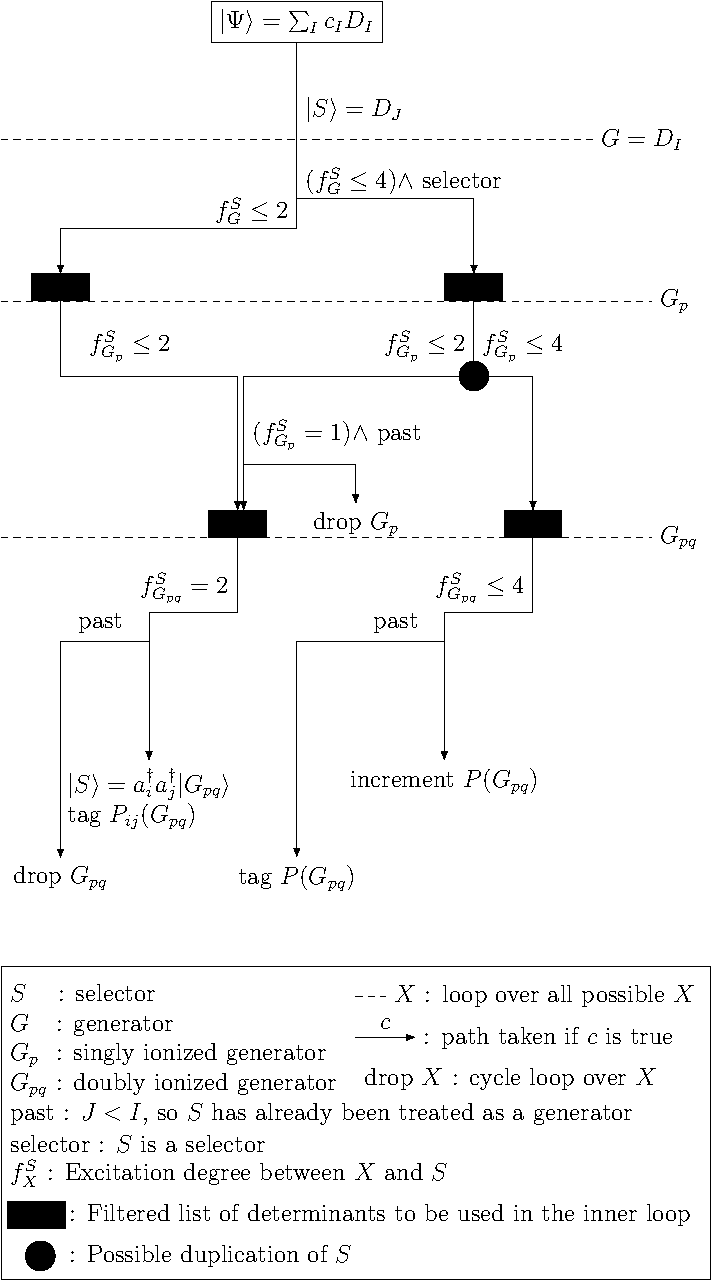
\includegraphics[height=0.90\textheight]{figures/cipsi/selection}
	\end{center}
        \caption{\label{fig:selection}
        $S$ is the selector currently flowing down the chart.
        Note that $M^{G_{pq}}$ is fully computed, and ``drop $G_{pq}$'' eventually reached, before any update is done to $P^{G_{pq}}$.
	}	
\end{figure}

Parallelisation \\
as seen, practical necessity to compute all alphas of the same generator at once \\
1 task = 1 generator, as simple \\

\end{document}
